\documentclass[]{article}
\usepackage{lmodern}
\usepackage{amssymb,amsmath}
\usepackage{ifxetex,ifluatex}
\usepackage{fixltx2e} % provides \textsubscript
\ifnum 0\ifxetex 1\fi\ifluatex 1\fi=0 % if pdftex
  \usepackage[T1]{fontenc}
  \usepackage[utf8]{inputenc}
\else % if luatex or xelatex
  \ifxetex
    \usepackage{mathspec}
  \else
    \usepackage{fontspec}
  \fi
  \defaultfontfeatures{Ligatures=TeX,Scale=MatchLowercase}
\fi
% use upquote if available, for straight quotes in verbatim environments
\IfFileExists{upquote.sty}{\usepackage{upquote}}{}
% use microtype if available
\IfFileExists{microtype.sty}{%
\usepackage{microtype}
\UseMicrotypeSet[protrusion]{basicmath} % disable protrusion for tt fonts
}{}
\usepackage[margin=1in]{geometry}
\usepackage{hyperref}
\PassOptionsToPackage{usenames,dvipsnames}{color} % color is loaded by hyperref
\hypersetup{unicode=true,
            pdftitle={Final Project - LSTM RNN Sales Demand Forecast},
            colorlinks=true,
            linkcolor=Maroon,
            citecolor=Blue,
            urlcolor=blue,
            breaklinks=true}
\urlstyle{same}  % don't use monospace font for urls
\usepackage{longtable,booktabs}
\usepackage{graphicx,grffile}
\makeatletter
\def\maxwidth{\ifdim\Gin@nat@width>\linewidth\linewidth\else\Gin@nat@width\fi}
\def\maxheight{\ifdim\Gin@nat@height>\textheight\textheight\else\Gin@nat@height\fi}
\makeatother
% Scale images if necessary, so that they will not overflow the page
% margins by default, and it is still possible to overwrite the defaults
% using explicit options in \includegraphics[width, height, ...]{}
\setkeys{Gin}{width=\maxwidth,height=\maxheight,keepaspectratio}
\IfFileExists{parskip.sty}{%
\usepackage{parskip}
}{% else
\setlength{\parindent}{0pt}
\setlength{\parskip}{6pt plus 2pt minus 1pt}
}
\setlength{\emergencystretch}{3em}  % prevent overfull lines
\providecommand{\tightlist}{%
  \setlength{\itemsep}{0pt}\setlength{\parskip}{0pt}}
\setcounter{secnumdepth}{0}
% Redefines (sub)paragraphs to behave more like sections
\ifx\paragraph\undefined\else
\let\oldparagraph\paragraph
\renewcommand{\paragraph}[1]{\oldparagraph{#1}\mbox{}}
\fi
\ifx\subparagraph\undefined\else
\let\oldsubparagraph\subparagraph
\renewcommand{\subparagraph}[1]{\oldsubparagraph{#1}\mbox{}}
\fi

%%% Use protect on footnotes to avoid problems with footnotes in titles
\let\rmarkdownfootnote\footnote%
\def\footnote{\protect\rmarkdownfootnote}

%%% Change title format to be more compact
\usepackage{titling}

% Create subtitle command for use in maketitle
\newcommand{\subtitle}[1]{
  \posttitle{
    \begin{center}\large#1\end{center}
    }
}

\setlength{\droptitle}{-2em}
  \title{Final Project - LSTM RNN Sales Demand Forecast}
  \pretitle{\vspace{\droptitle}\centering\huge}
  \posttitle{\par}
\subtitle{IA5008 Sistemas neuronales}
  \author{}
  \preauthor{}\postauthor{}
  \predate{\centering\large\emph}
  \postdate{\par}
  \date{Tuesday 8 May 2018}

\usepackage{float} \usepackage{caption}
\makeatletter\renewcommand*{\fps@figure}{H}\makeatother

\usepackage{amsthm}
\newtheorem{theorem}{Theorem}
\newtheorem{lemma}{Lemma}
\theoremstyle{definition}
\newtheorem{definition}{Definition}
\newtheorem{corollary}{Corollary}
\newtheorem{proposition}{Proposition}
\theoremstyle{definition}
\newtheorem{example}{Example}
\theoremstyle{definition}
\newtheorem{exercise}{Exercise}
\theoremstyle{remark}
\newtheorem*{remark}{Remark}
\newtheorem*{solution}{Solution}
\begin{document}
\maketitle
\begin{abstract}
Convenience stores are extremely constrained businesses with low profit
margins. Demand forecasting is one of the main exponents of their daily
planning toolbox. However, it is difficult to develop an effective
forecasting model that grasp temporal relationships without wasting
other valuable available features. Their most common and high quality
source of data are sales transactions. In this project we show the usage
LSTMs recurrent neural networks with highly encouraging results. Our
best result was a \(3*10^{-4}\) MAE for the overall unit predictions,
training by SKU sequences.
\end{abstract}

\textbf{Professor:} \href{mailto:vallejo@itesm.mx}{Edgar Emmanuel
Vallejo Clemente}

\textbf{Team Members:} \href{mailto:A01012491@itesm.mx}{Nisim Hurst,
A01012491}

\subsection{Introduction}\label{introduction}

\subsubsection{Problem description}\label{problem-description}

Convenience stores usually sell commodity products to people. These
products have an standard cost defined unilaterally by the manufacturer
targeting all the convenience stores regardless of brand, i.e.~whether
they are Oxxo, 7-Eleven, Gas Stations, etc. Also replenishment lapses
are subject to the manufacturer distribution network.

Given these constraints imposed by the multiple manufacturers, a
convenience store must manage to get it through by developing a strategy
usually based on one of the following key performance indicators: demand
forecasting, human resource management, fiscal strategies and real
estate management. For the purpose of this analysis we will focus on the
former: demand forecasting.

There are many hidden latent factors that are almost impossible to infer
from the usual sales transactions data alone, such as a store's location
and the manufacturers' marketing campaigns over that specific location.
Thus, being able to forecast product demand is extremely useful to:

\begin{itemize}
\tightlist
\item
  Update the economic order quantity to reduce stock and distribution
  costs.
\item
  Objectively evaluate a store's profit taking into account the
  forecasted demand and compare it with the other stores.
\item
  Develop pricing strategies based on price elasticity that maximize
  profit.
\end{itemize}

Price elasticity is a trivial and naïve attempt to forecast demand based
solely on price. Let \(Q\) be current units sold, \(P\) current price,
\(\Delta Q\) the change in quantity and \(\Delta P\) change in price.
Then, we define elasticity by the following formula: \[
e_p=\frac{\Delta Q}{\Delta P}*\frac{P}{Q}
\] This formula assumes that customers are rational beings and respond
to changes in prices by changing their buying preferences proportionally
to some degree. A negative elasticity coefficient evince customers buy
more at less price. When it is less than -1 it is considered to be a
relatively elastic demand at that point. Notice how the formula uses the
current price-quantity pair to calculate the elasticity at some given
level. So, in reality this formula may yield an hyperbolic convex curve
rather than just a linear slope.

To calculate price elasticity from sales transactions alone is an
grueling task, though. The source of these data are not controlled
pricing experiments. Thus, to assume the variation in price is exogenous
is way to risky and the basic assumption for parameter identification of
the least square method is broken. Also, right price strategies are
difficult to predict because most of the products are subject to
behavioral economics variables like the
\href{https://en.wikipedia.org/wiki/Veblen_good}{Veblen Effect}
{[}\protect\hyperlink{ref-Veblen}{1}{]} , i.e.~when the elasticity is
positive, or changes in demographics that are outside of the scope of
the data. Price elasticity models are usually designed by a human and
optimized by a machine, but nowadays these models are falling short
behind the velocity of global economic changes.

Yet, there are still ways to forecast demand with an acceptable
confidence interval. One of the most common ones is the
\href{https://en.wikipedia.org/wiki/Autoregressive_integrated_moving_average}{ARIMA
model} {[}\protect\hyperlink{ref-Hyndman}{2}{]}. It stands for
autoregressive integrated moving average model. The most outstanding
feature of this model is that it uses the same variable at lag times for
both input and output. The probability is not always assumed to be
necessarily stationary so it can cope seamlessly with seasonality
trends. Despite these clear advantages, using it makes more difficult to
take into account other factors apart from the demand out-of-the-shelf.

\href{https://en.wikipedia.org/wiki/Hidden_Markov_model}{Hidden Markov
models} are Bayesian temporal models that can help us infer latent
variables and handle product sales sequences of variable length.
Nonetheless, they fall in the stationary probability assumption. Also,
they fail to capture long term relationships between the data because of
the Markov assumption that a future state is only dependent of the
immediately previous state. Also, on Markov chains you have to find a
way to compress the whole problem into one variable only.

Neural networks are deterministic models that can be used for both
regression and autoregression tasks. An added advantage is that
hierarchical features are unsupervisedly built from other categorical
predictors without leaving behind temporal relations. Densely connected
simple multilayer perceptron neural networks are good when the i.d.d.
(independent and identically distributed) assumption holds. However,
when data is correlated in time or space is a bit trickier to deal with.

Recurrent neural networks have emerged as an effective and scalable
models for sequential data. However, they can't deal with product sales
sequences of variable length. A way to overcome this limitation is by
using sequence padding to the max length. Long Short-Term memory neural
networks are a kind of recurrent neural that introduce a memory cell
which can maintain its state over time, and non-linear gating units
which regulate the information flow into and out of the cell
{[}\protect\hyperlink{ref-Greff2017}{3}{]}.

Thus, we propose a LSTM-based method that could meet all the challenges
listed above. Namely, we would like to estimate units sold using an
automatically learned price elasticity model.

LSTM basic elements are: 1. memory cell, 2. input gate, 3. output gate
and 4. forget gate. For a complete introduction please refer to
{[}\protect\hyperlink{ref-Greff2017}{3}{]}.

\subsubsection{Questions to answer}\label{questions-to-answer}

\begin{enumerate}
\def\labelenumi{\arabic{enumi}.}
\tightlist
\item
  \textbf{Can this dataset be used to train a recurrent neural network
  that produces over 60\% accuracy on the predicted 1 month horizon?} Is
  the data sufficient? are there any bayes error bounds implicit in the
  data?
\item
  \textbf{How similar products sales relate to the data?} can we use
  data of one product category (human labeled) and use it to predict the
  units sold of another category? can we use a kind of transfer learning
  from other pre-trained datasets?
\item
  \textbf{Is there any seasonality for some products?} are there any
  periodic elements that would affect the units sold regardless of the
  other variables.
\item
  \textbf{How elastic are the products?} how changes in prices and other
  ancillary variables affect the units sold.
\end{enumerate}

Further details of the dataset where provided on a previous project
proposal. However, the dataset was extracted from the article
{[}\protect\hyperlink{ref-Hervert-Escobar2017}{4}{]} by Laura
Hervert-Escobar of the \emph{Instituto Tecnológico y de Estudios
Superiores de Monterrey}. The original objective of this dataset was to
find a pricing optimization model from some features suggested by the
business's executives. The data was provided from a real retail store
business, so it has some rights reserved and discretion is advised.

\subsubsection{Assumptions and
hypothesis}\label{assumptions-and-hypothesis}

We assume the following:

\begin{enumerate}
\def\labelenumi{\arabic{enumi}.}
\tightlist
\item
  If a row doesn't appear in the dataset we assume there was no sale of
  that product on that day. Thus, sampling was made evenly through the
  year.
\item
  If a product haven't appeared in the series until some point of or if
  it doesn't appears any more since some point, the past assumption
  doesn't hold for those intervals.
\item
  There are non-workable holydays that explain the lack of data on some
  periods.
\item
  Some holyday weekends have no data for all the products, we assume we
  can fill those points with the last measured value per product, even
  if they are marked as zero.
\item
  Climate conditions are independent of all other variables but can be a
  dependable variable for units.
\item
  Cost is independent of all other variables but can be a dependable
  variable for price both internal and of the competitors.
\end{enumerate}

Under this conditions, we are confident to be able to build a
multivariate time series forecasting model with LSTM which can predict
demand based on the following variables:

\begin{itemize}
\tightlist
\item
  \textbf{Input}

  \begin{itemize}
  \tightlist
  \item
    \textbf{Prices.} How changes in prices affect demand?
  \item
    \textbf{Cost.} Are there any suppliers trends related to time?
  \item
    \textbf{Climate.} Can climate changes trigger or hinder sales? Are
    there any trends in the climate that we can predict regardless of
    the other variables?
  \end{itemize}
\item
  \textbf{Target}

  \begin{itemize}
  \tightlist
  \item
    \textbf{Units.} How are the units affected by all the other
    variables?
  \end{itemize}
\end{itemize}

Each SKU is meant to be a sequence of sales for our model to predict the
demand. The max sequence length is 93, i.e.~the maximum number of weeks
sampled.

\subsection{Methodology}\label{methodology}

\subsubsection{State-of-the-art review}\label{state-of-the-art-review}

In {[}\protect\hyperlink{ref-Kochak2015}{5}{]}, the authors also took
and ANN MLP approach and recomend it over other methods such as ARIMA.
They observed that as forecasting periods becomes smaller, using ANN
provides more accuracy in the forecast. They also had less than 2 years
of data to train so, this work quite resemble ours in extensions.

In conjunction with the classical \emph{Mean Absolute Error} (MAE), and
its scaled version \emph{Mean Absolute Percentage Error} (MAPE), we will
also use the \emph{Mean Squared Logarithmic Error} (MSLE) as proposed by
{[}\protect\hyperlink{ref-Taghizadeh2017}{6}{]} which is given by the
formula:

\[
\sqrt{\frac{1}{n}\sum_{i=1}^{n}(\log(p_i+1)-\log(a_i+1))^2}
\]

Where \(p_i\) is the predicted value for sample \(i\) and \(a_i\) is the
actual or real value. This metric has the advantage that even highly
fluctuating unit range per SKU also give consistent results.

\subsubsection{Data exploration and
preprocessing}\label{data-exploration-and-preprocessing}

The dimensions of this dataset consist on: 78578 samples, 15 features,
1030 unique sku (sequences), 70 categories. There are about 14 sku sales
sequences per category. The data is spread out evenly over a period of
93 continuous weeks.

\paragraph{Seasonality trends}\label{seasonality-trends}

Autoregressive models use the data of one variable of the previous step
to predict that same variable. Are the \emph{units} feature we are
trying to predict a proper feature to predict using autoregression?
Well, lag plots allow to detect those kind of relationships through time
in the date. Lets see how it behaves:

\begin{figure}

{\centering 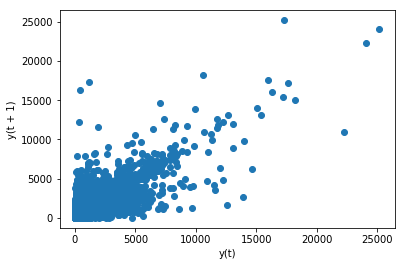
\includegraphics[width=0.4\linewidth]{./media/lag_plot} 

}

\caption{Pandas Lag Plot}\label{fig:fig1}
\end{figure}

We can see from Figure \ref{fig:fig1} that there is a clear linear
correlation relationship that we can use to construct a regression model
out of just these periodic changes in the \emph{units} feature.

So, we can conclude from this graph that by using the \emph{units}
predictor we will increase our models' accuracy and it favors the
autoregression approach.

\paragraph{Data cleansing at column
level}\label{data-cleansing-at-column-level}

From the module \texttt{sklearn.feature\_selection} we used
\texttt{SelectKBest} and \texttt{f\_regression} to see which other
variables are important to the regression task over the \emph{units}
feature\footnote{This model is slightly better than a simple linear
  correlation and a good explanation can be found on
  \href{https://stats.stackexchange.com/questions/204141/difference-between-selecting-features-based-on-f-regression-and-based-on-r2}{stackoverflow}}
:

\begin{longtable}[]{@{}rrll@{}}
\caption{\label{tab:tab1} Features' F-Score for predicting
\emph{units}}\tabularnewline
\toprule
F Score & P Value & Support & Attribute\tabularnewline
\midrule
\endfirsthead
\toprule
F Score & P Value & Support & Attribute\tabularnewline
\midrule
\endhead
6097.77 & 0 & True & PROMOTION\tabularnewline
4883.87 & 0 & True & SYSTEM PRICE\tabularnewline
4234.03 & 0 & True & REAL PRICE\tabularnewline
3680.61 & 0 & True & NetCost\tabularnewline
2047.72 & 0 & True & Competitor's price\tabularnewline
1675.34 & 0 & False & SKU\tabularnewline
777.626 & 2.68519e-170 & False & CATEGORY\tabularnewline
60.0118 & 9.54124e-15 & False & WEEK\tabularnewline
46.0613 & 1.15421e-11 & False & MIN TEMP\tabularnewline
3.62565 & 0.056899 & False & AVG TEMP\tabularnewline
2.6292 & 0.104919 & False & RAIN INTENSITY\tabularnewline
1.78562 & 0.181465 & False & MAX TEMP\tabularnewline
\bottomrule
\end{longtable}

We can see from Table \ref{tab:tab1} that one of the best feature to
predict \emph{units} is if the item has or hasn't \emph{promotion}. This
can be easily explain by taking into account that seller grant promotion
to increase sales volume. \emph{System price} is the second most
influent variable followed by \emph{real price} and since only 19
products have a mean absolute elasticity lower or equal than one
(following a kind of Veblen effect) we can confidently say the products
are \textbf{elastic}.

So, if we would like to use the orthogonalization method and reduce
overfiting after achieving a good accuracy, we could just drop the
features that have a low F-Score, i.e.~those from \emph{week} to
\emph{max-temp}.

Related to elasticity is cross elasticity of demand
{[}\protect\hyperlink{ref-Frank2014}{7}{]}. This effect is also called
cannibalization and it happens when an item begins to steal the sales of
a similar item of the same category and price. Here is a list of
products that may be victims of cannibalization:

\begin{longtable}[]{@{}rrrrrr@{}}
\caption{\label{tab:tab2} Cannibalization items}\tabularnewline
\toprule
sku1 & sku2 & correlation & cat1 & price1 & price2\tabularnewline
\midrule
\endfirsthead
\toprule
sku1 & sku2 & correlation & cat1 & price1 & price2\tabularnewline
\midrule
\endhead
793 & 797 & -0.888922 & 20 & 14.8572 & 16.065\tabularnewline
735 & 797 & -0.882422 & 20 & 16.8941 & 16.065\tabularnewline
1204 & 1209 & -0.80364 & 30 & 17.305 & 18.3708\tabularnewline
734 & 797 & -0.802659 & 20 & 14.2464 & 16.065\tabularnewline
1208 & 1209 & -0.796488 & 30 & 20.5644 & 18.3708\tabularnewline
1207 & 1209 & -0.775419 & 30 & 22.4275 & 18.3708\tabularnewline
298 & 305 & -0.721268 & 50 & 25.5154 & 20.5474\tabularnewline
1201 & 1206 & -0.685368 & 30 & 15.8318 & 13.3298\tabularnewline
745 & 797 & -0.667326 & 20 & 13.9792 & 16.065\tabularnewline
724 & 797 & -0.666368 & 20 & 13.8644 & 16.065\tabularnewline
287 & 289 & -0.636817 & 41 & 10.0019 & 10.9023\tabularnewline
\bottomrule
\end{longtable}

These items represent less than \%0.632746 of the total sales so we can
safely ignore them. An advantage of the neural network is that this kind
of relationship between items are automatically learned and the only
thing we must ensure is that these effect is balanced or diminished to
some insignificant degree.

\paragraph{Data cleansing at row
level}\label{data-cleansing-at-row-level}

For each product, we have up to 93 observations, one per week. This
limits the applicability of some machine learning models which need more
data. Trying to find some seasonality in the data is also difficult,
since we have less than two years of information. This leaves us with
581 out of 1030 products. All these product sequences can be trivially
fed to the LSTM. However, for the other 449 products we would need some
kind of padding.

An equally important observation is that data is not scaled down between
0 and 1 for a good performance of the neural network. On RNN Batch
Normalization can't be used since the statistics are computed per batch,
i.e.~weights are shared per batch. So, we will make use of an extra
prepossesing step using the \emph{MinMaxScaler} module from the
\emph{sklearn.preprocessing} package.

\subsection{Experiments}\label{experiments}

Two approaches were tested, one generative of all the possible sequences
since some starting point and the other by using just 1 step lag values.
However, common parameter were set up for comparison on both approaches:

\begin{enumerate}
\def\labelenumi{\arabic{enumi}.}
\tightlist
\item
  \emph{ADAM} as optimizer
\item
  Default learning rate of \(0.001\)
\item
  50 LSTM units
\item
  50 epochs
\item
  Batch size of 72
\item
  1 final unit of a densely connected layer was used to concentrate the
  output into single a regression neuron
\end{enumerate}

\subsubsection{Approach 1. Padding sequences per
SKU}\label{approach-1.-padding-sequences-per-sku}

The first approach\footnote{based on this
  \href{https://stackoverflow.com/questions/39674713/neural-network-lstm-input-shape-from-dataframe}{answer}}
generated sequences for each SKU by progressively taking more sequence
elements until reaching the max sequence length. First each row is
transformed into a single input vector which represents a value on the
sequence. So we will start from the one that has 1 length and all zeros
to the last one having all the 93 items extracted from the data. A
sequence for each of the of the 1030 items, multiplied by the padding of
a max length of 93 sequences gave a total of 95,790 sequences. This
quantity was extremely high and training took so long that had to be
cancelled.

\begin{figure}

{\centering 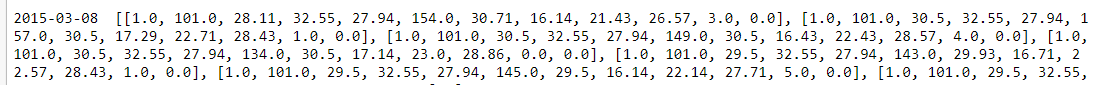
\includegraphics[width=0.3\linewidth]{./media/example_representation1} 

}

\caption{Representation example of cummulative vectors}\label{fig:fig3}
\end{figure}

Then, we tried by just leaving the 581 items that have presence over all
the 93 weeks. Just 581 was specially detrimental for the networks
performance. Finally, we tried to filter out the items that didn't had
the longest sequence per item. So, there were only 1030 sequences left
for training. This quantity was also too low and didn't achieve good
results.

\begin{figure}

{\centering 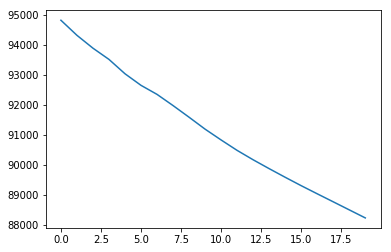
\includegraphics[width=0.3\linewidth]{./media/app2.2} 

}

\caption{MSE for the padding approach (still too high)}\label{fig:fig2}
\end{figure}

That approach didn't gave good results so there was no point in
exploring it further.

\subsubsection{Approach 2. Using lag values of a previous
state}\label{approach-2.-using-lag-values-of-a-previous-state}

The second approach\footnote{based on this
  \href{https://machinelearningmastery.com/multivariate-time-series-forecasting-lstms-keras/}{blog}}
was to treat each transaction record as a sequence composed by the
immediately previous record for that item. Thus, we will have a 2 states
fixed length sequence for each record. Having 13 predictors this yields
a total of 25 features, the ones of the previous and the ones of the
current state excluding the units that is the variable we are trying to
predict.

\begin{figure}

{\centering 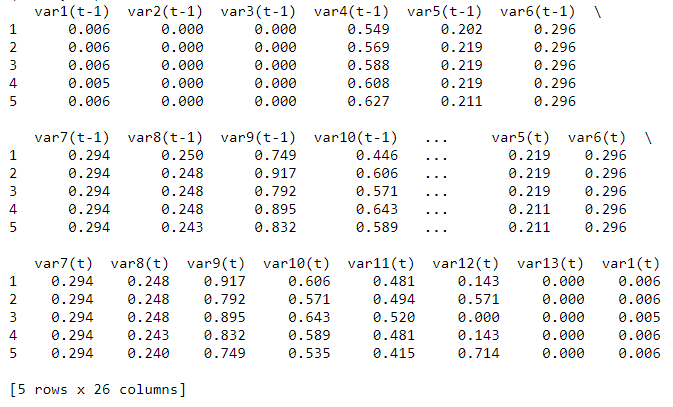
\includegraphics[width=0.5\linewidth]{./media/example_representation2} 

}

\caption{Horizontal stack of two consecutive sales records for a given product, already normalized between 0 and 1}\label{fig:fig4}
\end{figure}

Figure \ref{fig:fig4} show the representation already scaled using the
\emph{MinMaxScaler} function and horizontally stacked for the first 5
pairs of sequences. Coincidentally they belong to the same item.

Given that this problem is about regression we cant user stratified
K-Fold. So, the most we can do is to split the dataset randomly several
times and average their results.

A first test was made by calculating the lag on each separated
\emph{SKU}, assuming distinct \emph{SKU's} would have distinct trends.
However, by doing this we inadvertently filtered out all the product
sales records that didn't had a previous record. So, from a total of
78578 records it leave us with only 77548 (-1030). These were the
results:

\begin{figure}

{\centering 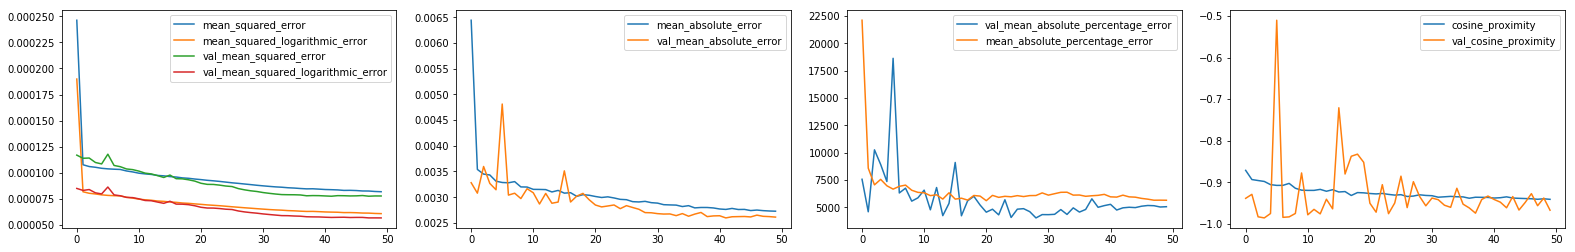
\includegraphics[width=1\linewidth]{./media/res_1} 

}

\caption{Results between train a validation sets for several metrics}\label{fig:fig5}
\end{figure}\begin{figure}

{\centering 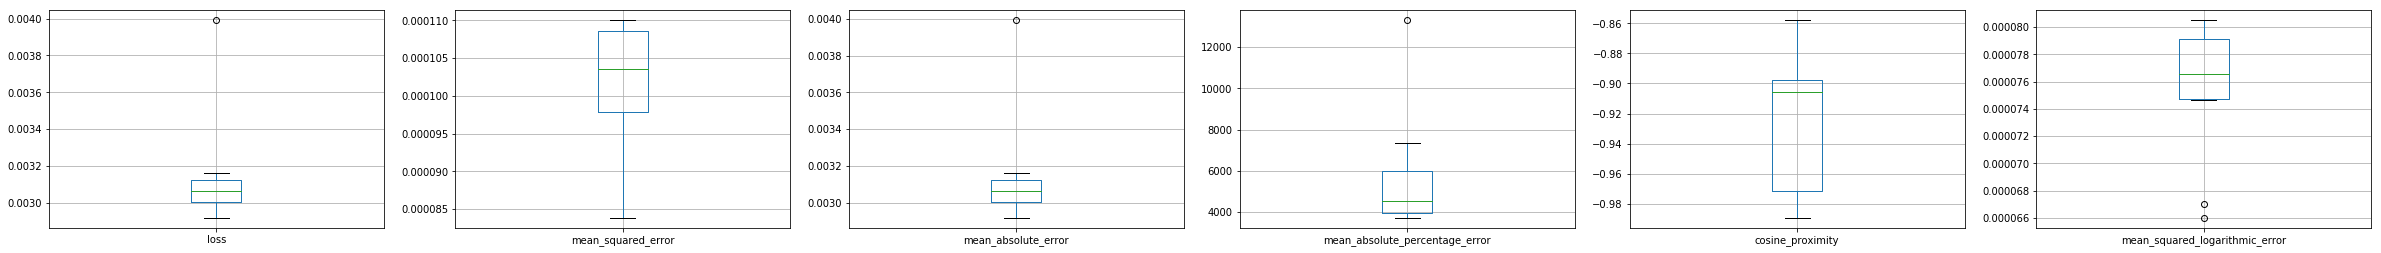
\includegraphics[width=1\linewidth]{./media/box_1} 

}

\caption{Box plots for analysis of variance over 10 random splits}\label{fig:fig6}
\end{figure}

From Figure \ref{fig:fig5} we see that the data is sufficient to
generate a learning curve that shows 20 epochs would be enough for the
network to learn temporal relationships. From the boxplots we see that
surprisingly, the most stable accuracy measure is the MSE. The median
MSE value is considerably lower than the one achieved by the first
approach, i.e.~8800 vs 0.0001.

\begin{figure}

{\centering 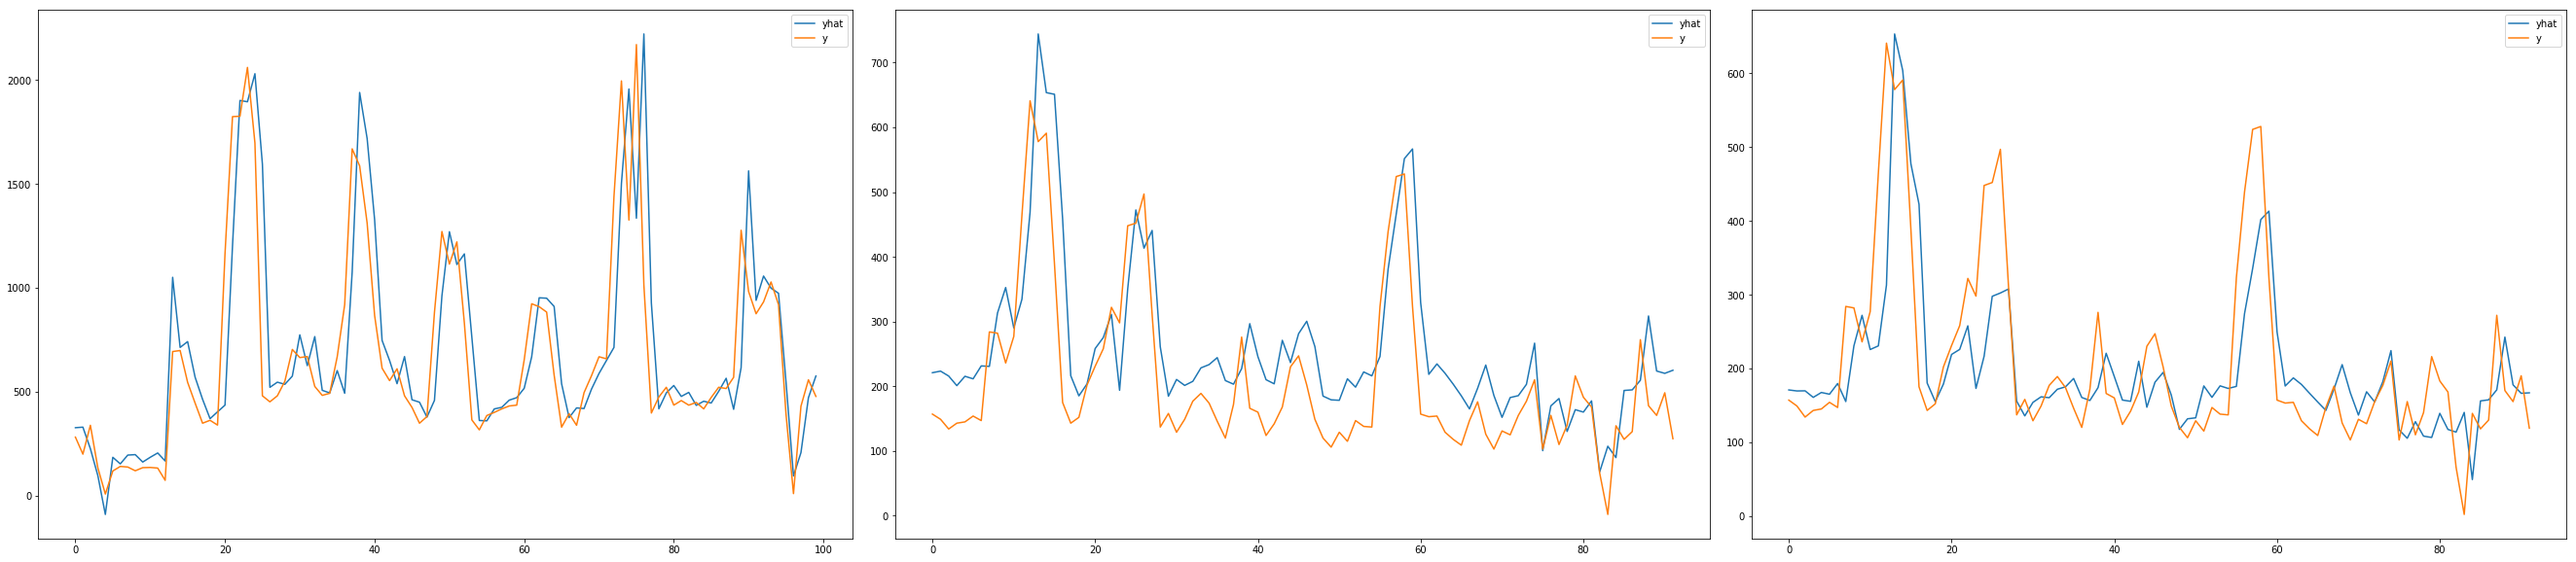
\includegraphics[width=0.8\linewidth]{./media/pred} 

}

\caption{1. Prediction over all SKU units; 2. one item and; 3. the same item with a price increase of 10 perc.}\label{fig:fig7}
\end{figure}

The left most tile of Figure \ref{fig:fig7} shows the prediction for all
the items demand over the full range of 93 weeks, then for only one
product and finally for the same product but with a 10\% price increase.
We can see our hypothesis that a LSTM can help us build a successful
elasticity model is confirmed. On the general prediction we see that the
predicted units are close to the real units and is yielding results
comparable to ARIMA of Figure \ref{fig:fig8} for \(\frac{1}{3}\) of the
weeks, i.e.~32 samples.

\begin{figure}

{\centering 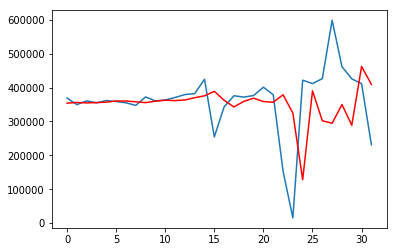
\includegraphics[width=0.3\linewidth]{./media/arima2} 

}

\caption{$(5,1,0)$ ARIMA reference model for the sum of the units un the last third of the data}\label{fig:fig8}
\end{figure}

The other 2 predictions by product show how the model is capturing
elasticity relationships that are directly reflected on the predicted
\emph{units} to be sold.

We also tried to remove the SKU column and predict by just the other
variables:

\begin{figure}

{\centering 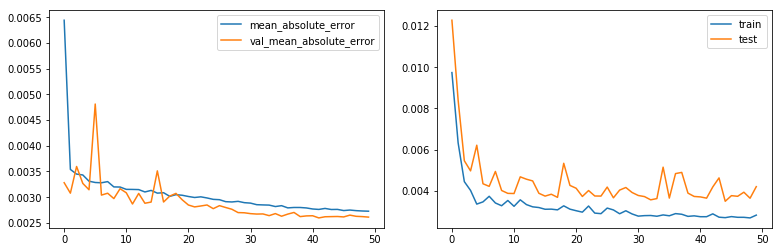
\includegraphics[width=0.7\linewidth]{./media/side_cat} 

}

\caption{Side-by-side comparison between training by SKU and training by category}\label{fig:fig9}
\end{figure}

The left hand side image of Figure \ref{fig:fig9} is the same learning
curve using \emph{SKU} and the other side is the one that just has the
other columns except \emph{SKU}. We can see they still remain on the
same order of magnitude even though the one that used the \emph{SKU} has
a lower MAE because it is using particular trends of each \emph{SKU}.

Finally, we tried to test what amount of loss could reduced by using one
more time step of lag values for the series\footnote{A total of two
  timesteps that remove 2060 records from the dataset. Train on 51267
  samples, validate on 25252 = 76519} :

\begin{figure}

{\centering 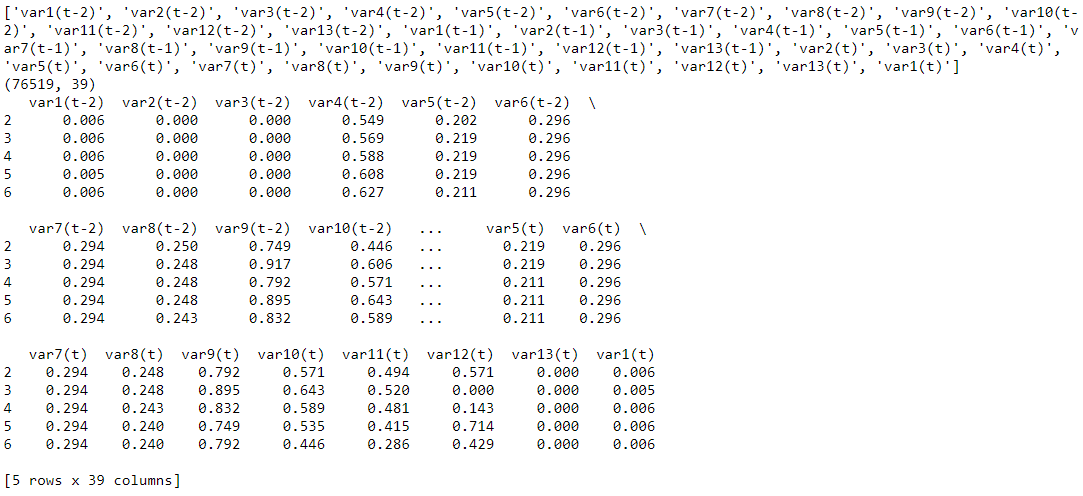
\includegraphics[width=0.5\linewidth]{./media/example_representation3} 

}

\caption{Second representation with more timesteps in the same row}\label{fig:fig10}
\end{figure}

\begin{figure}

{\centering 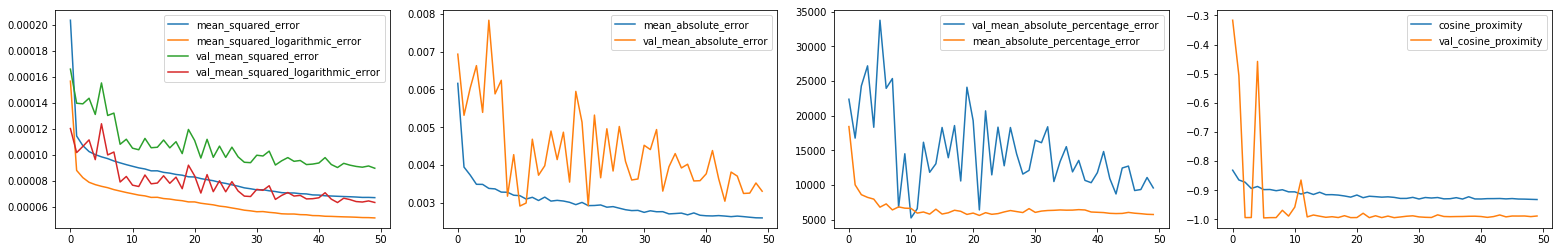
\includegraphics[width=1\linewidth]{./media/res_2} 

}

\caption{Results with a timestep of 2}\label{fig:fig11}
\end{figure}

Figure \ref{fig:fig11} shows extremely similiar results were obtained
between the previous 1-timestep test and the actual 2-timesteps test,
yielding the same order of magnitude for each metric used. Nonetheless,
we see a surprising behavior in which the variance of \emph{MAE} and
\emph{MAEP} increases for the test set. However, due lack of time, we
didn't get to do variance analysis to validate if the those steep jumps
remains over all the training splits.

\subsubsection{Implementation details}\label{implementation-details}

The Keras python notebook implementation was tested using a Quadro M500M
with 384 CUDA cores at 1080MHz with 2GB memory and 1 CPU of 2.81 GHz.
The whole process took about 1 hour 40 minutes to train (8 seconds per
epoch over 50 epochs times 10 random splits).

\subsection{Results discussion}\label{results-discussion}

Here is a summary of some important empirical observations based on the
previous \nameref{experiments} section:

\begin{enumerate}
\def\labelenumi{\arabic{enumi}.}
\tightlist
\item
  Dimensionality reduction was never required because the difference
  between training and validation sets performance wasn't too important.
  However, maybe feature work could focus on varying the number of
  epochs to a bigger order of magnitude and see if it is convenient.
\item
  A lag plot evinced that this task could be neatly treated using an
  auto regression approach, so we tried a naïve ARIMA. However, by
  considering all the other predictors, on the current and on the
  previous time step, LSTM was able to outperform ARIMA.
\item
  The first approach of generating vector embedding's concatenating the
  values of each row and then stack them by item to predict \emph{units}
  hinted a deficiency in the method used. This can be explained by the
  fact that we drastically reduced the total number of samples that were
  fed into the LSTM from roughly \(7.8*10^4\) to 1030.
\item
  The second approach yielded better results almost immediately, even
  with less epochs. It was verified that just relying on the previous
  state was sufficient to detect short term temporal relations, so using
  a hidden Markov model would probably have given similar results.
\item
  Random splits showed that the most consistent metric to use was
  \emph{MAE}, confirming our state-of-the-art review.
\item
  Including the SKU predictor on the training features yielded slightly
  better loss results, but not much significant, just about 20\% better
  on \emph{MAE} but the learning curve retained the same shape.
\item
  Including more timesteps in the representation gave contradictory
  results. We would expect more accurate predictions, however the
  variance of some of \emph{MAE} and \emph{MAPE} metrics (our champions
  by the way) just go through the roof. This suggest further examination
  of this phenomenon with more epochs or varying the hyperparameters is
  required.
\end{enumerate}

\subsection{Conclusions}\label{conclusions}

In this work successfully predicted demand units from the previous time
step and all the other available variables using an LSTM and achieving a
competitive result of on \(3*10^{-4}\) \emph{MAE}. We empirically
corroborate, that even when the available data wasn't covering too much
time (only 93 weeks), the LSTM performed better than ARIMA as suggested
in the paper of {[}\protect\hyperlink{ref-Kochak2015}{5}{]}.

An elasticity model was able to be inferred from the data even when
there is a small percent of items that are subject to the
cannibalization effect (about 16 of 1030). This elasticity model was
proven to respond as expected given a 10\% point price increase.

Thus, this model can be used confidently in online prediction of
\emph{unit's} demand given the assumption that missing values in the
data are properly filled by the last known \emph{units} quantity, lest
the model learns an unexplainable leap from zero to some arbitrary
level.

\subsection*{References}\label{references}
\addcontentsline{toc}{subsection}{References}

\hypertarget{refs}{}
\hypertarget{ref-Veblen}{}
{[}1{]} T. Veblen, ``The Theory of the Leisure Class.''

\hypertarget{ref-Hyndman}{}
{[}2{]} R. J. Hyndman and G. Athanasopoulos, \emph{Forecasting :
principles and practice}. p. 291.

\hypertarget{ref-Greff2017}{}
{[}3{]} K. Greff, R. K. Srivastava, J. Koutnik, B. R. Steunebrink, and
J. Schmidhuber, ``LSTM: A Search Space Odyssey,'' \emph{IEEE
Transactions on Neural Networks and Learning Systems}, vol. 28, no. 10,
pp. 2222--2232, 2017.

\hypertarget{ref-Hervert-Escobar2017}{}
{[}4{]} L. Hervert-Escobar, O. A. Esquivel-Flores, and R. V.
Ramirez-Velarde, ``Optimal pricing model based on reduction dimension: A
case of study for convenience stores,'' \emph{Procedia Computer
Science}, vol. 108, pp. 2079--2089, 2017.

\hypertarget{ref-Kochak2015}{}
{[}5{]} A. Kochak and S. Sharma, ``Demand Forecasting Using Neural
Network for Supply Chain Management,'' \emph{International Journal of
Mechanical Engineering and Robotics Research}, vol. 4, no. 1, pp.
96--104, 2015.

\hypertarget{ref-Taghizadeh2017}{}
{[}6{]} E. Taghizadeh, ``Utilizing artificial neural networks to predict
demand for weather-sensitive products at retail stores,'' 2017.

\hypertarget{ref-Frank2014}{}
{[}7{]} R. Frank, \emph{Microeconomics and behavior.} Irwin Mcgraw-Hill,
2014.


\end{document}
